\documentclass{article}

\usepackage[margin=2.5cm,left=2cm,includefoot]{geometry}
\usepackage{graphicx}
\usepackage{float}
\usepackage[space]{grffile}
\usepackage{hyperref}
\usepackage[export]{adjustbox}
\usepackage{multicol}
\usepackage{caption}
\usepackage{hyperref}
\usepackage{listings}
\usepackage{vhistory}
\usepackage{titlesec}

\setcounter{secnumdepth}{4}

\titleformat{\paragraph}
{\normalfont\normalsize\bfseries}{\theparagraph}{1em}{}
\titlespacing*{\paragraph}
{0pt}{3.25ex plus 1ex minus .2ex}{1.5ex plus .2ex}

% Header and footer
\usepackage{fancyhdr}
\pagestyle{fancy}

\rhead{COS301}
\lhead{Testing Document}
\fancyfoot[R]{Page \thepage}

\renewcommand{\headrulewidth}{2pt}
\renewcommand{\footrulewidth}{1pt}

\begin{document}

	\begin{titlepage}
		\begin{center}
			
\includegraphics[width=10cm]{images/UP.jpg}  \\
			[0.5cm]
			\huge{
			Testing Document\\
			}
			
			\line(1,0){300}\\
			[0.2cm]
			\LARGE{Project: Insurance profiling from social media\\
			Client: RetroRabbit} \\
			\line(1,0){300}\\
			\LARGE{Team: Valknut Solutions}\\
			[1.0cm]
			\large{Version: 1.0}\\
			[1.0cm]
			\large
			{
			\begin{itemize}
				\item 13054903 - Charl Jansen van Vuuren 
				\item 10297902 - Bernhard Schuld      
				\item 13044924 - Kevin Heritage
				\item 13176545 - Quinton Weenink\\
			\end{itemize}
			}
			\textsc{\large}\\
		[3.0cm]
		\textsc{\large  Department of Computer Science}\\
		[0.5cm]
		\textsc{\large \today}\\
		\end{center}
	\end{titlepage}
	
	\cleardoublepage
	% Start of the revision history table
	\begin{versionhistory}
  		\vhEntry{1.0}{27.7.2016}{CJvV,KH,QW}{created}
	\end{versionhistory}	
	
	\cleardoublepage
	\tableofcontents
	\cleardoublepage
	
\section{Introduction}
This document contains information related to Testing of the Insurance Profiling project that is being developed for RetroRabbit as part of the COS301 module at the University Of Pretoria. \\
This document is based on the IEEE 829 Standard for Testing Documentation \href{http://www.fit.vutbr.cz/study/courses/ITS/public/ieee829.html}{IEEE 829}

\section{References to other documentation}
\begin{itemize}
	\item{Requirements specifications as per 29 July 2016}
	\item{Architecture Design as per 29 July 2016}
\end{itemize}

\section{Test items}
The items included in this test document includes:
\begin{itemize}
	\item Backend API calls
	\item Database management functions
	\item Environmental tests 
	\item Deployment and compatibility tests
\end{itemize} 

\section{Features to be Tested}
These include features to be tested are rated based on the level or risk associated namely, High (H), Medium (M) and Low (L).

\begin{itemize}
\item API calls to do:
	\begin{itemize}
	\item Database insertions (H)
	\item Database deletions (H)
	\item Database retrievals (L)
	\end{itemize}
\item Environmental test
	\begin{itemize}
	\item Integration test to determine the current environment (development or deployment) to react accordingly (M)
	\end{itemize}
\item Deployment/Build testing including Compatibility
		\begin{itemize}
	\item Automated testing by the Travis CI framework to ensure the current feature is compatible with different versions of the NodeJS framework. (H)
	\end{itemize}
\end{itemize}

\cleardoublepage
\section{Features not to be Tested}
\begin{itemize}
	\item Email functionality
	\begin{itemize}
		\item This feature didn't form part of the previous sprint and is not yet in use.
		\item Testing is not yet needed or this feature
	\end{itemize}
	\item The ability to receive data from a Facebook lead ad cannot be tested but this data has been mocked to ensure proper integration testing.
	\item Front-end features including:
	\begin{itemize}
		\item Analyst login
		\item Authentication
	\end{itemize}
\end{itemize}

\section{Approach (Strategy)}
\begin{itemize}
	\item The testing framework Mocha will be used to run unit tests at compilation time or per request.
	\item Deployment and compatibility testing is done with the automated framework Travis CI. Travis ensures all changes made to a branch is compatible with the different versions of NodeJS and the current environment (development or deployment).
	\item A number of developed unit tests will be run with Mocha as can be seen in Figure \ref{fig:MochaTests}.
	\item The testing of Facebook lead data was mocked out to be testable. 
	\item The use of Postman to test API routes manually, ie. to make POST requests. Postman is a browser extension developed for API testing.
	\item The current compatibility tests include Node version 6.2 and 5.11 
\end{itemize}


\section{Running tests}
Tests can be ran with the command "npm test" which will run Mocha, if this test is run locally it will connect to the local database.
Travis CI runs these test to the external database hosted on Heroku. The Travis tests are ran when a new branch is merged to ensure compatibility with all versions of Node.
\section{Item Pass/Fail Criteria for Tests}
If the specified Pre-condition is not met the test will fail. \\
If the specified Post-condition is met the test will pass.
\cleardoublepage
\section{Tests}
\subsection{The following tests all passed as intended:}
\begin{itemize}
\item Creating row in Database - POST : /api/user/ 
	\begin{itemize}
	\item Pre-conditions:
		\begin{itemize}
		\item Database is connected and created
		\item The following values are specified:  
		\begin{itemize}
		\item firstName
  		\item lastName
  		\item mobileNumber 
  		\item maritalStatus 
  		\item dateOfBirth 
 		\item gender
  		\item location 
 		\item email
 		\end{itemize} 
		\end{itemize}
	\item Post-condition - The row gets persisted
	\item Figure \ref{fig:MochaTests}
	\end{itemize}

\item Retrieving row in Database based on currentUser - GET : /api/user/:currentUser
	\begin{itemize}
	\item Pre-condition - The currentUser exists
	\item Post-condition - The currentUser is retrieved 
	\item Figure \ref{fig:MochaTests}
	\end{itemize}
	
\item Removing row in Database based on currentUser - DELETE : /api/user/:currentUser
	\begin{itemize}
	\item Pre-condition - The currentUser exists
	\item Post-condition - The currentUser is removed 
	\item Figure \ref{fig:MochaTests}
	\end{itemize}	
	\begin{figure}[H]
  	\centering
      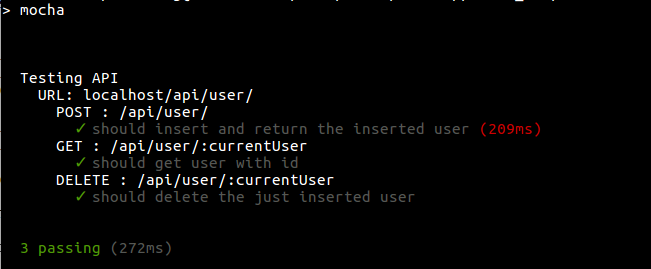
\includegraphics[width=\textwidth]{images/tests.png}
  	\caption{Output of Mocha tests}
  	\label{fig:MochaTests}
	\end{figure}


\item Travis CI build test for Node version 5.11
	\begin{itemize}
	\item Pre-condition - The changes to the branch are compatible with version 5.11
	\item Post-condition - The build will pass successfully 
	\item Figure \ref{fig:5_11}
	\end{itemize}	
	
	\begin{figure}[h]
  	\centering
      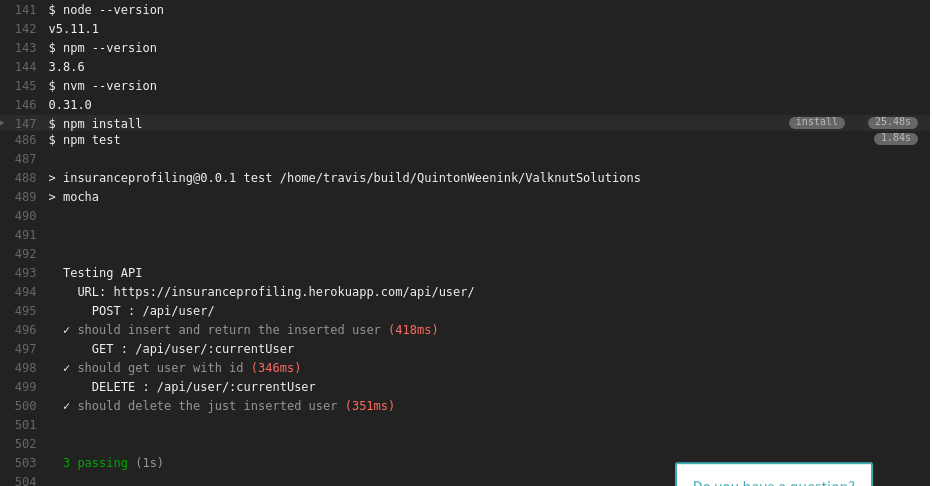
\includegraphics[width=\textwidth]{images/5_11.png}
  	\caption{Output of Travis tests for Node version 5.11}
  	\label{fig:5_11}
	\end{figure}

\cleardoublepage
\item Travis CI build test for Node version 6.2
	\begin{itemize}
	\item Pre-condition - The changes to the branch are compatible with version 6.2
	\item Post-condition - The build will pass successfully 
	\item Figure \ref{fig:6_2}
	\end{itemize}	
\end{itemize}

\begin{figure}[h]
  \centering
      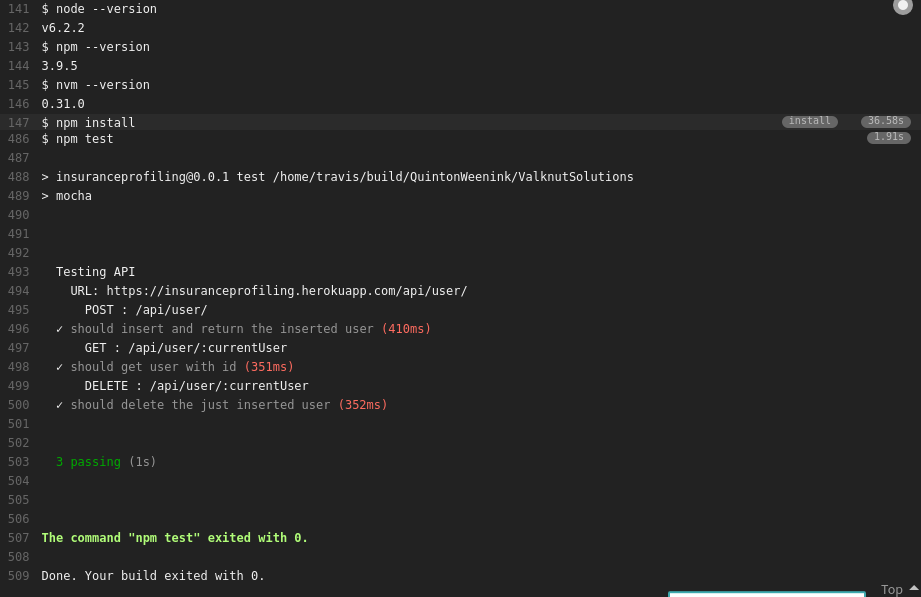
\includegraphics[width=\textwidth]{images/6_2.png}
  \caption{Output of Travis tests for Node version 6.2}
  \label{fig:6_2}
\end{figure}


\cleardoublepage
\subsection{The following tests failed as intended:}
\begin{itemize}
	\item Travis CI build, running Mocha when a branch was merged.
	\begin{itemize}
	\item Pre-condition - Heroku server is online.
	\item Post-condition - The build will pass successfully 
	\item Figure \ref{fig:failed}
	\item This test failed as a result of the hosting server being offline, not fulfilling the Pre-condition. 
	\item The error stating a timeout proves this failure.
	\end{itemize}

	\begin{figure}[h]
  	\centering
      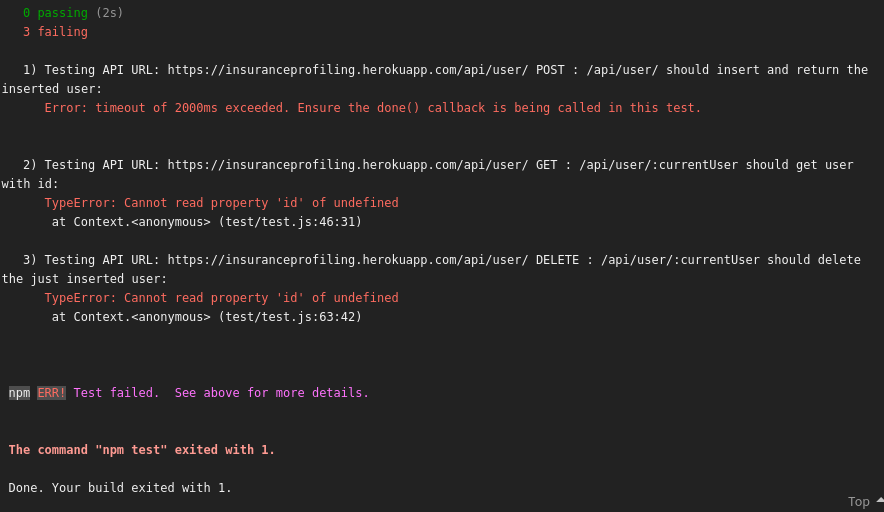
\includegraphics[width=\textwidth]{images/failed.png}
  	\caption{Output of failed Travis test}
  	\label{fig:failed}
	\end{figure}	
	
	\cleardoublepage
	\item Database connection test based on Mocha test
	\begin{itemize}
	\item Pre-conditions
	\begin{itemize}
		\item The database exists and is created
		\item The database accepts connections
	\end{itemize}
	\item Post-condition - The test will pass
	\item Figure \ref{fig:DBFailed}
	\item This test failed as a the Pre-conditions did not hold. 
	\item The database was not initialized at that time.
	\end{itemize}


	\begin{figure}[h]
  	\centering
      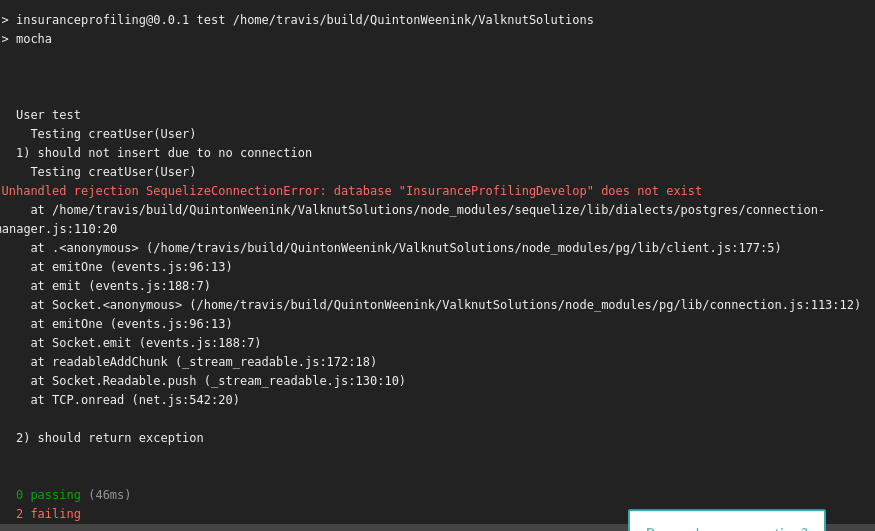
\includegraphics[width=\textwidth]{images/DBConnectionFailed.png}
  	\caption{Database connection test}
  	\label{fig:DBFailed}
	\end{figure}	
	
	
	\begin{figure}[h]
  	\centering
      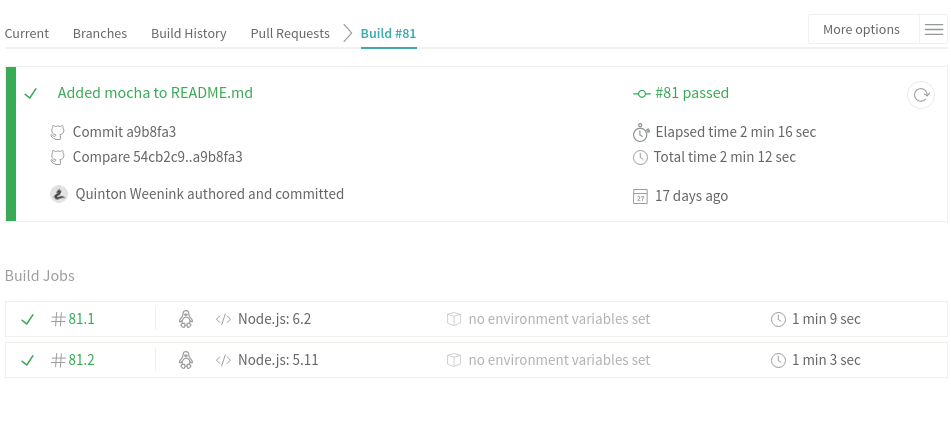
\includegraphics[width=\textwidth]{images/TravisInterface.png}
  	\caption{Travis interface used for test logs}
	\end{figure}

\end{itemize}

\cleardoublepage
\section{Test Summary}
This project follows a Continous Integration model with regards to testing. \\ Any new feature to be merged with the main branch is first tested, then reviewed by the person merging the branch and only then the merge is closed.\\
The amount of tests are limited in the current version of the system, this is as a result of the complexity of testing external API calls,such as Facebook, on which our system heavily relies.\\
Future versions will include more tests based on these complexities.

\end{document}
